\documentclass[10pt]{article}
\usepackage[polish]{babel}
\usepackage[utf8]{inputenc}
\usepackage[T1]{fontenc}
\usepackage{amsmath}
\usepackage{amsfonts}
\usepackage{amssymb}
\usepackage[version=4]{mhchem}
\usepackage{stmaryrd}
\usepackage{graphicx}
\usepackage[export]{adjustbox}
\graphicspath{ {./images/} }

\title{Sprawdzian predyspozycji }

\author{}
\date{}


\begin{document}
\maketitle
Czerwiec 2012

\section*{Zadanie 1}
Oblicz, ile jest dwunastocyfrowych liczb naturalnych, których iloczyn cyfr jest równy 6. Odpowiedź uzasadnij.

\section*{Zadanie 2}
Wykaż, że jeżeli \(0<a_{1}<a_{2}<a_{3}<a_{4}<a_{5}<a_{6}\), to \(\frac{a_{1}+a_{2}+a_{3}+a_{4}+a_{5}+a_{6}}{a_{3}+a_{6}}<3\).

\section*{Zadanie 3}
Dane są liczby całkowite \(a, b\) takie, że liczba \(6 a+11 b\) jest podzielna przez 31. Wykaż, że liczba \(a+7 b\) także jest podzielna przez 31 .

\section*{Zadanie 4}
Czy istnieje taki trójkąt ostrokątny, w którym długości dwóch boków są liczbami niewymiernymi, a długość trzeciego boku i pole są liczbami wymiernymi? Odpowiedź uzasadnij.

\section*{Zadanie 5}
W trójkącie \(A B C\) punkt \(E\) należy do boku \(B C\), punkt \(M\) jest środkiem odcinka \(A E\). Proste \(A B\) i MC przecinają się w punkcie \(F\). Wykaż, że pole trójkąta \(M E C\) jest większe od pola trójkąta \(M A F\).

\section*{Zadanie 6}
Dany jest sześcian, jak na rysunku. Długość krawędzi sześcianu jest równa 1 . Od sześcianu odcięto czworościany APQS oraz BQRP. Oblicz objętość otrzymanego wielościanu.\\
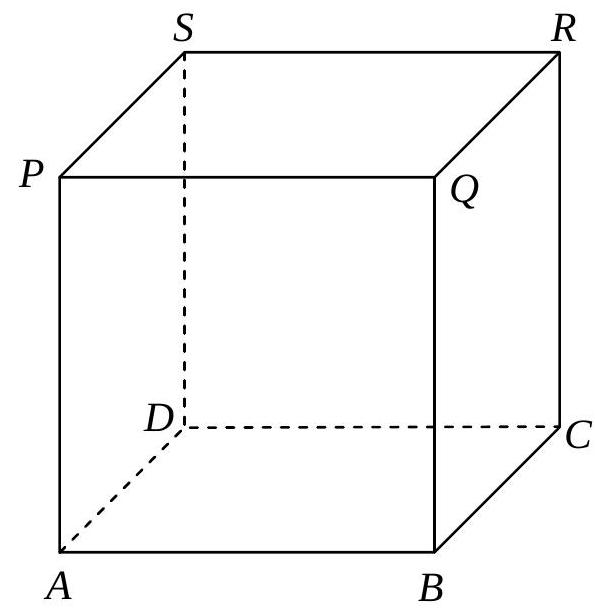
\includegraphics[max width=\textwidth, center]{2024_11_21_8eddb11774ef9ec7d4a6g-1}

Powodzenia


\end{document}